\documentclass[a4paper,10pt,twoside]{article}
%%%%%%%%%%% Packages %%%%%%%%%%
\usepackage[margin=1in]{geometry}
\usepackage{amsmath, amssymb,mathtools}
\usepackage{fancyhdr}
\usepackage{sectsty}
\usepackage{graphicx,wrapfig}
\usepackage{enumitem}
\usepackage{float}
\usepackage{braket}
\usepackage{bbm}
\usepackage{tikz,calc}
\usepackage{amsthm}


%%%%%%%%%%% Macros %%%%%%%%%%
\def \note#1 {\vspace{-1em}\paragraph{\bfseries #1}}
\def \dd {{\rm d}}
\def \id {{\mathbbm{1}}}
\def \order {\mathcal{O}}
\def\bquad{\mkern-18mu}
\DeclareMathOperator{\trace}{tr}
\DeclareMathOperator{\spanset}{span}

%%%%%%%%%%% Tikz Definitions %%%%%%%%%%
\usetikzlibrary{shapes, arrows,positioning,fit}
\tikzstyle{plain} = [draw,thick,circle,inner sep=0,minimum size=0.5cm,font=\footnotesize]
\tikzstyle{mps} = [draw,thick,rectangle,rounded corners=.1cm,inner sep=0,minimum size=0.5cm]
\tikzstyle{mpo} = [draw,thick,circle,inner sep=0,minimum size=0.5cm]
\tikzstyle{index} = [-,thick,font=\footnotesize]
\tikzstyle{virtual} = [-,thick,dotted,font=\footnotesize]

\def \tu {0.25cm}

%%%%%%%%%%% Formatting %%%%%%%%%%
\pagestyle{fancy}
\renewcommand{\footrulewidth}{0.5pt}

\fancyhf{}
\lhead{04/05/2017}
\chead{Quantum Information Methods in Many-Body Physics}
\rhead{PH2269}
\lfoot{Giacomo Giudice~~~~giacomo.giudice@mpq.mpg.de}
\rfoot{Page \thepage}

\allsectionsfont{\normalfont\sffamily}

\newtheoremstyle{modern}{3pt}{3pt}{\itshape}{}{\sffamily\bfseries}{}{.5em}{}
\theoremstyle{modern}
\newtheorem{lemma}{Lemma}[section]
\newtheorem{theorem}[lemma]{Theorem}

%%%%%%%%%%% Here Begins Document %%%%%%%%%%
\begin{document}
\title{\vspace{-1cm}\sffamily Homework 3\vspace{-1cm}}
\author{}
\date{}
\maketitle
\thispagestyle{fancy}


\begin{section}{The Fundamental Theorem of MPS}
Let $A$ be an injective tensor generating some translationally-invariant matrix product state $\ket{\Psi_A}$.
Write down explicitly the overlap, and show --- this time without diagrammatic notation --- that
\[
  \braket{{\Psi}_A|{\Psi}_A}  = \trace\left( 
  {
  \tikz[baseline=-1.5*\tu]{
    \node[mps] at (\tu,0.5*\tu) (upper) {$\bar{A}$};
    \node[mps,below=\tu of upper] (lower) {$A$};
    \draw[index] (upper.west) -- +(-\tu,0);
    \draw[index] (upper.east) -- +(\tu,0);
    \draw[index] (lower.west) -- +(-\tu,0);
    \draw[index] (lower.east) -- +(\tu,0);
    \draw[index] (lower.north) -- (upper.south);
    \useasboundingbox (0,-0.5*\tu) rectangle (1*\tu,0.5*\tu);
    }
  }
 \right)^N = \trace{\mathbb{E}^N},
\]
where $\mathbb{E} = \sum_i \bar{A}^i \otimes A^i$ is the \emph{transfer matrix}.
We can associate to it two linear maps, $\varepsilon$, as well as its adjoint $\varepsilon^*$ (by looking at the matrix from the other direction)
\[
  \varepsilon(\sigma) = \sum_i A^i \sigma {A^i}^\dag, \quad \varepsilon^*(\sigma) = \sum_i {A^i}^\dag  \sigma A^i,
\]
\note{Hint} You might find the following property useful: $ \trace(A\otimes B) = \trace A \trace B$.

Without loss of generality, we can take the spectral radius of the transfer matrix to  be unity (we can always achieve that by rescaling $A$).
Let $\ket{r}$ and $\bra{\ell}$ be the dominant right and left eigenvectors, respectively, of  $\mathbb{E}$. 
It can be shown that $r$ and $\ell$ correspond to the fixed points of the associated linear maps $\varepsilon$ and $\varepsilon^*$, and they are both positive\footnote{D. E. Evans and E. H{\o}egh-Krohn, J. London Math. Soc. 17, 345-355 (1978). See Thm. 2.5.}.
Additionally, for injective tensors, $r$ and $\ell$ are full rank and strictly positive definite.
Show that the gauge transformation $\tilde{A}^i = XA^i X^{-1}$, with $X = \sqrt{1/r}$ brings $A$ in its right-canonical form ($\sum_i \tilde{A}^i \tilde{A}^{i\dag} = \id$), while the gauge $X = \sqrt{\ell}$ gives the left-canonical form\footnote{These forms are possible even without injectivity. It is slightly harder to show, since $A$ needs to be decomposed in blocks. See D. Per{\'e}z-Garc{\'i}a, F. Verstraete, M.M. Wolf and J.I. Cirac, arXiv:0608197 (2006).} ($\sum_i \tilde{A}^{i\dag} \tilde{A}^i = \id$).
Choosing the left-canonical form, we then have $\rho = \ell$, and the fixed points of the maps are
\[
  \varepsilon(\rho) = \rho ,\quad \varepsilon^*(\id) = \id.
\]
Write down the diagrammatic expression corresponding to these equations.

\begin{theorem}[Fundamental theorem of MPS]
Given two MPS characterized by the injective tensors $A$ and $B$, then $\ket{\Psi_A} = \ket{\Psi_B}$, as $N \to \infty$, if and only if there exists a gauge transform $X$ which relates $A$ and $B$ as $X A^i= B^i X$.
\end{theorem}

You shall now prove this theorem. 
The backwards direction (``$\Leftarrow$'') should be immediately clear.
Let us now look at the forward direction (``$\Rightarrow$'') of the theorem.
Assume the states are correctly normalized, hence  $\ket{\Psi_A} = \ket{\Psi_B} \Leftrightarrow |\braket{\Psi_A|\Psi_B}|=1$.

Now define the operator
\[
   \braket{{\Psi}_B|{\Psi}_A} = \trace \mathbb{E}_{\rm rel}^N
\]
Let $X$ be the dominant eigenvector of $\mathbb{E}_{\rm rel}$ with eigenvalue $\lambda$.
What are the maximum value of $|\lambda|$?
How does it determine the overlap $\braket{{\Psi}_B|{\Psi}_A}$ in the thermodynamic limit?
The eigenvalue equation for its associated linear map reads $\varepsilon_{\rm rel}^\ast(X) = \sum_i B^{i\dag} X A^i = \lambda X$. 
Now, without loss of generality, we can take $A$ and $B$ to be in canonical form. 
Use the Cauchy--Schwarz inequality $ |\braket{u|v}|^2 \leq \| u \|^2\| v \|^2$ to show that
\[
   \left|\lambda \trace(X \rho X^\dag)\right|^2 \leq \left(\sum_i \trace(X A^i \rho {A^i}^\dag X^\dag)\right) \! \left(\sum_i \trace(B^i X \rho X^\dag {B^i}^\dag)\right) = \left| \trace(X \rho X^\dag)\right|^2
\]
You may use equations, diagrammatic expressions, or a combination of both.
When is the Cauchy-Schwarz inequality an equality? 
In that case, conclude by showing that $X A^i= B^i X$.
\note{Hint} The trick is to think of the trace as an overlap: $\trace(u^\dag v) =  \braket{u|v}$.
\end{section}

\begin{section}{The AKLT State, Once Again}
In the last homework we derived the tensor for the AKLT state $\ket{\Psi} = \sum_{\boldsymbol{\sigma}} \trace{\left(A^{\sigma_1} A^{\sigma_2} \dots A^{\sigma_L}\right)} \ket{\boldsymbol{\sigma}}$, with
\[
  A^+=\frac{1}{\sqrt{2}}
  \begin{pmatrix}
    0 & 1\\
    0 & 0
  \end{pmatrix}, \quad
  A^0=\frac{1}{2}
  \begin{pmatrix}
    -1 & 0\\
    0 & 1
  \end{pmatrix}, \quad
  A^-=\frac{1}{\sqrt{2}}
  \begin{pmatrix}
    0 & 0\\
    -1 & 0
  \end{pmatrix}.
\]
Rescale the matrices such that $\sum_\sigma {A^\sigma}^\dag A^\sigma = \id$, to obtain the left-canonical form.
Compute the transfer matrix and its eigenvalues (numerically, if you want).
Check that in the limit $L \to \infty$, $\| \Psi \|^2 = 1$.
\end{section}

\begin{section}{A Non-Injective MPS}
Recall that  the GHZ state is generated by the tensor $A^i = \delta_{i,a,b}$, $i = 0,1$.
Show that for any blocking of length $L$ (see the next exercise for a definition), the subspace $\mathcal{S}_L$ of the GHZ state contains only two linearly independent vectors.
Deduce that one cannot obtain an injective tensor after blocking for any finite $L$. 
Hence $A$ cannot be a so-called \emph{normal} tensor.


Compute the transfer matrix.
Notice that there are two distinct dominant eigenvectors, let us call them $\ket{\rho_\uparrow}$ and $\ket{\rho_\downarrow}$.
What is $\braket{{\rm GHZ} | {\rm GHZ}}$ as a function of $N$?
Let $O_n$ be a \emph{local} operator acting on site $n$.
Calculate the expectation values 
\[
  \braket{\cdot} = \frac{\braket{\psi | \cdot | \psi}}{\braket{\psi|\psi}}
\]
for $\psi = {\rm GHZ}$ of the following observables, in terms of the matrix $\mathbb{E}_O = \sum_{i,j} O_{ij} (\bar{A}^i \otimes A^j)$:
\begin{itemize}
  \item $\braket{O_n}$,
  \item $C_L = \braket{O_n O_{L+n}} - \braket{O_n}\braket{O_{L+n}} $,
\end{itemize}
Does the correlation go to zero as $L \to \infty$?
\end{section}

\begin{section}{Uniqueness of the Ground State for Parent Hamiltonians}
Let $\ket{\Psi}$ be an MPS generated by an \emph{injective} tensor $A$.
The \emph{blocking} operation over $k$ sites is the map
\[
  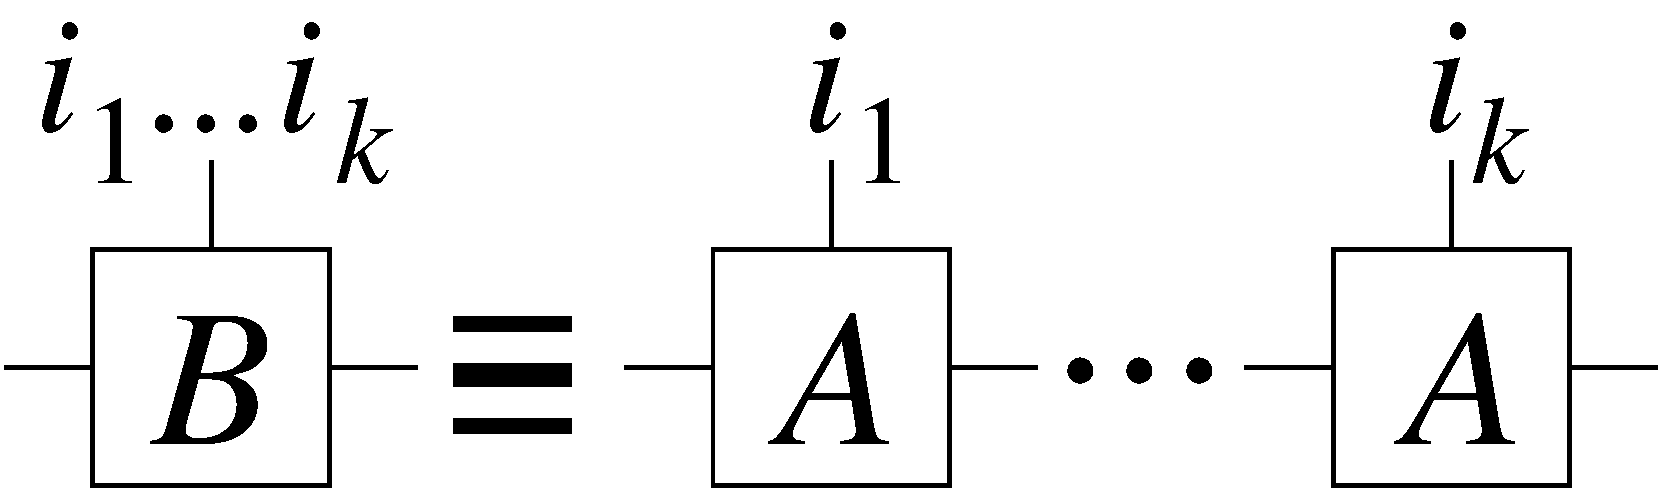
\includegraphics[height=2.5em]{diagrams/block-tens}
\]
Verify the stability of the injectivity condition under blocking --- that means, show that the superblock obtained by blocking $k$ tensors still has the injectivity property (modulo a constant).
There are a couple ways of doing this, you can use a diagrammatic argument,
or you can use the mathematical definition of injectivity, namely that the map $X \mapsto \sum_i \trace(A^i X) \ket{i}$ is injective.

In this exercise we will prove the uniqueness of parent Hamiltonians, for \emph{injective} tensors. 
To keep thing simple, we will restrict out attention to the one dimension, in the case where the parent Hamiltonian is a sum of \emph{nearest-neighbor} terms $h_{i,i+1}$.
Therefore we define the subspace
\[
  \mathcal S_2=\left\{ \sum_{i,j}\trace(A^iA^jX)\ket{i,j} \middle\vert X\in\mathbf{L}(\mathbb{C}^{D \times D}) \right\} =
    \left\{\raisebox{-1.7em}{\,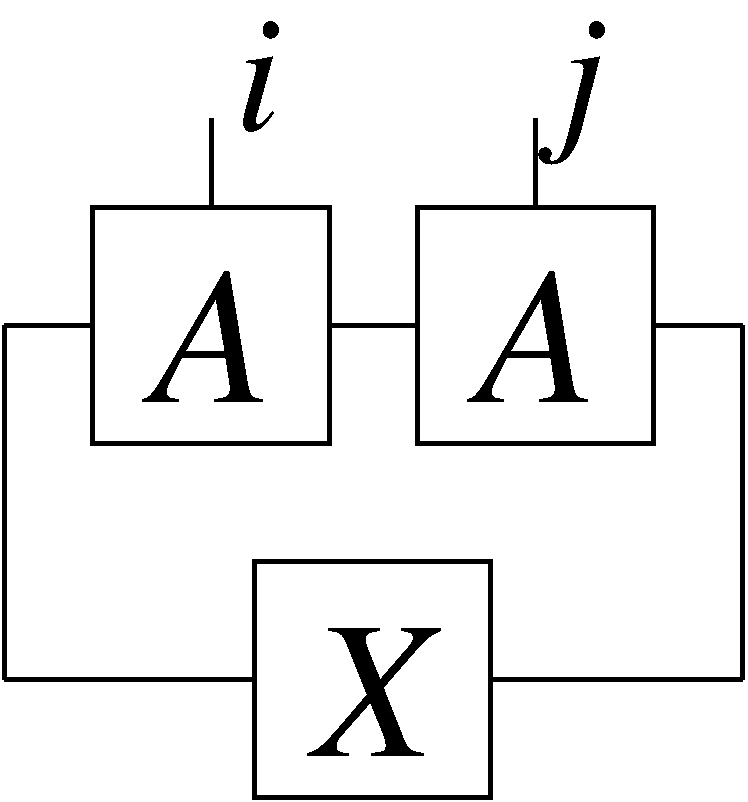
\includegraphics[height=4em]{diagrams/trBBX}}\ \,\middle\vert X\in \mathbf{L}(\mathbb{C}^{D \times D}) \right\}.
\]
where $\mathbf{L}(\mathbb{C}^{D \times D})$ is the space of all $D \times D$ matrices over $\mathbb{C}$.
This space is just a special case of a series of subspaces
\[
  \mathcal{S}_k = \left\{\sum_{i_1,\dots,i_k}  \trace(A^{i_1} \dots A^{i_k} X) \ket{i_1,\dots,i_k}\ \,\middle\vert X \in \mathbf{L}(\mathbb{C}^{D \times D})\right\}.
\]
Show that $\mathcal{S}_k$ is the range of the $k$-sites reduced density matrix $\rho_k$.

Let me remind you of how you obtain the parent Hamiltonian: by defining the projector onto the space orthogonal to $\mathcal{S}_2$, we can construct the local term $h_{i,i+1}$.
The parent Hamiltonian is then simply the sum of these local terms, $H = \sum_i h_{i,i+1}$.

In order to prove the uniqueness, we will start by considering a chain with open boundary conditions, and show that the ground state subspace is $\mathcal{S}_2$.
We will then close the boundaries, and show that the only state remaining is $\ket{\Psi}$.
We can formalize this with two theorems.

\begin{theorem}[Intersection property]
\label{thm:intersection}
Let $A$ and $B$ be injective tensors.
Then,
\[
    \left\{\raisebox{-1.7em}{\,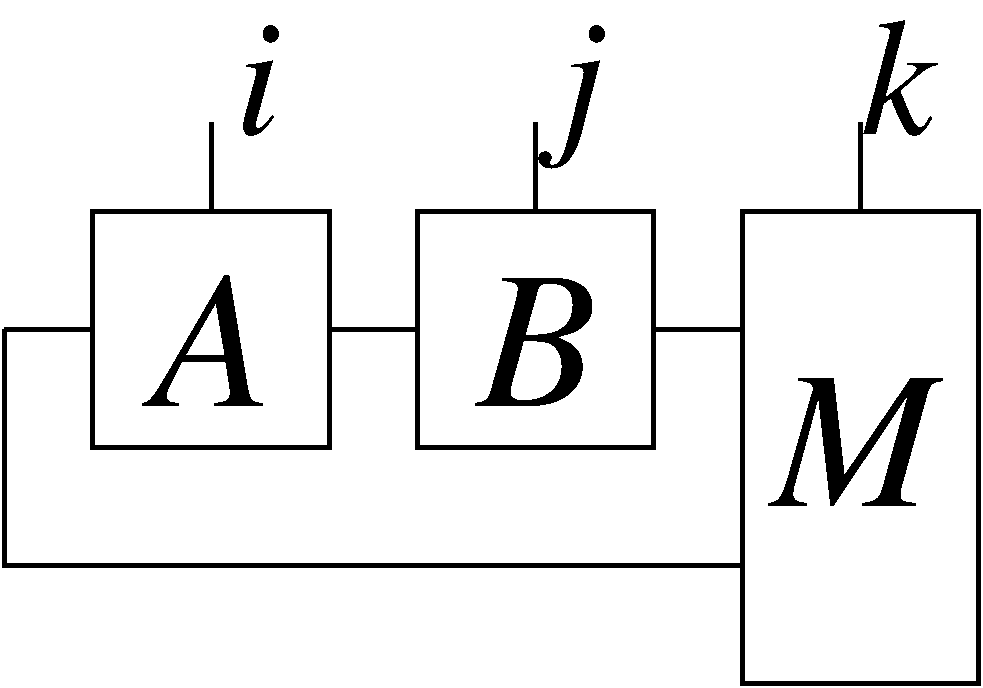
\includegraphics[height=4em]{diagrams/trBBM}}\ \,\middle\vert \ M \right\}
    \cap
    \left\{\raisebox{-1.7em}{\,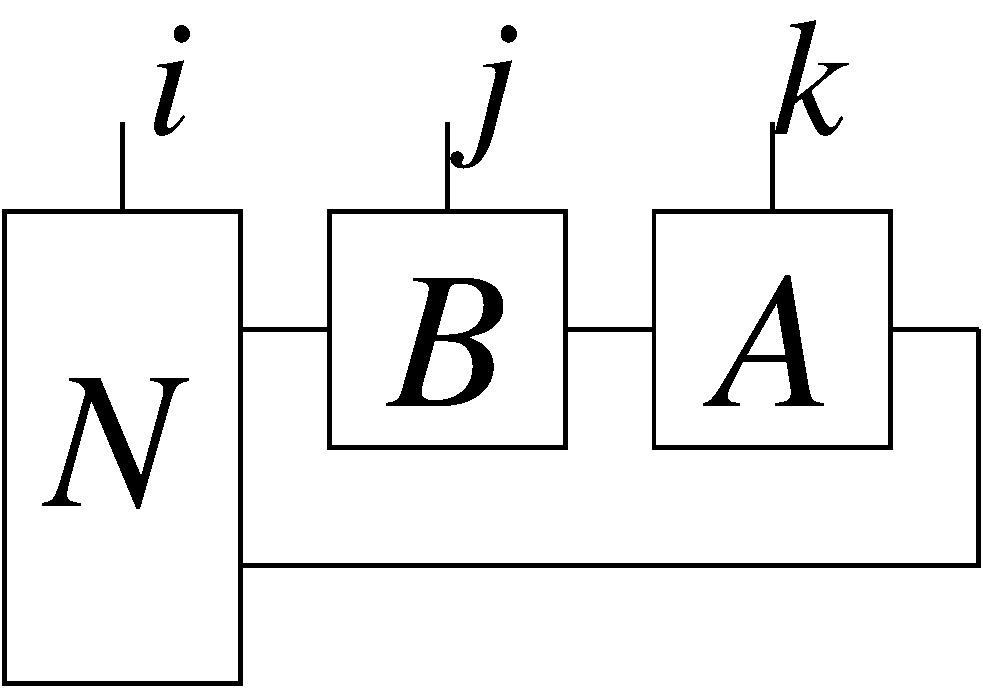
\includegraphics[height=4em]{diagrams/trNBB}}\ \,\middle\vert \ N \right\}=
    \left\{\raisebox{-1.7em}{\,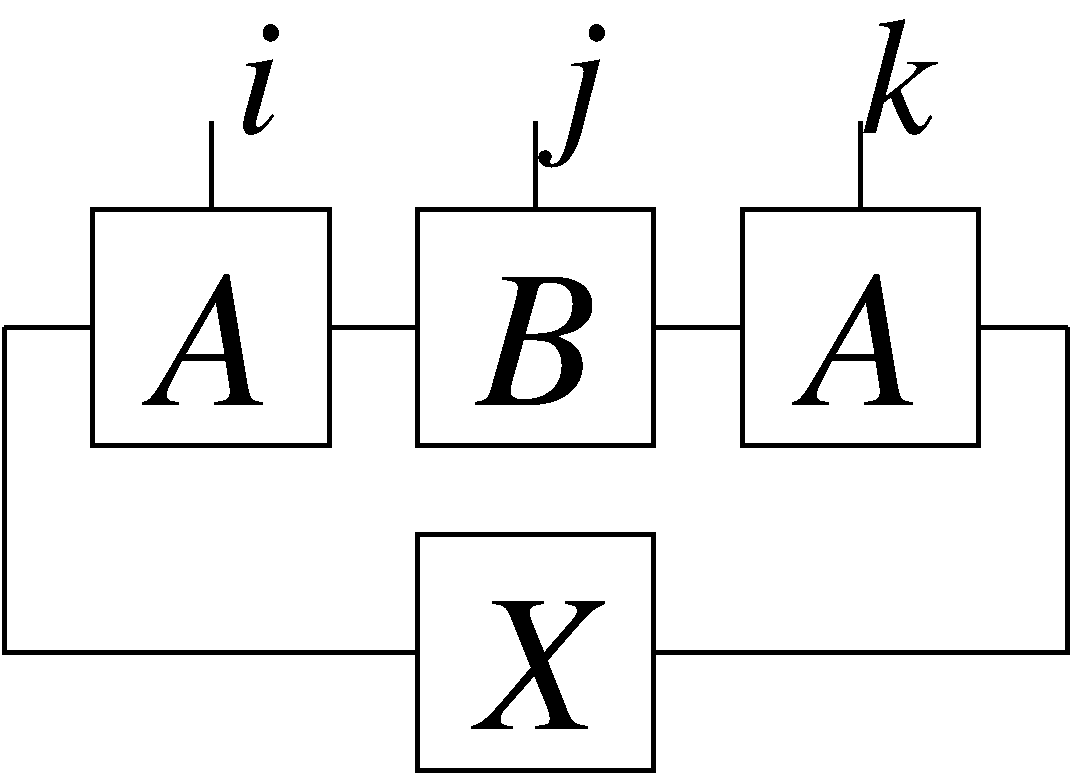
\includegraphics[height=4em]{diagrams/trBBB}}\ \,\middle\vert \ X \right\},
\]
with $M$, $N$, $X \in \mathbf{L}(\mathbb{C}^{D \times D})$.
\end{theorem}

We shall prove this theorem by showing inclusion in both directions.
Construct a state in the right hand side that belongs in both of the other two sets on the left hand side.
Conversely, for any state $\ket{\psi}$ in the l.h.s., there exists $M$, $N$ such that
\[
    \ket{\psi}=
    \raisebox{-1.7em}{\,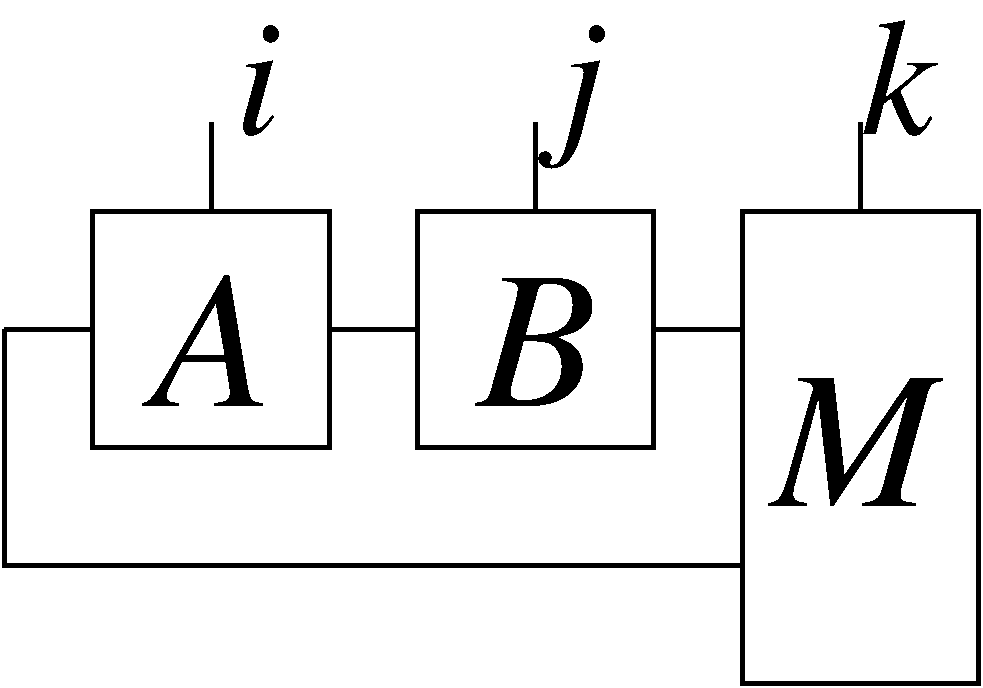
\includegraphics[height=4em]{diagrams/trBBM}} =
    \raisebox{-1.7em}{\,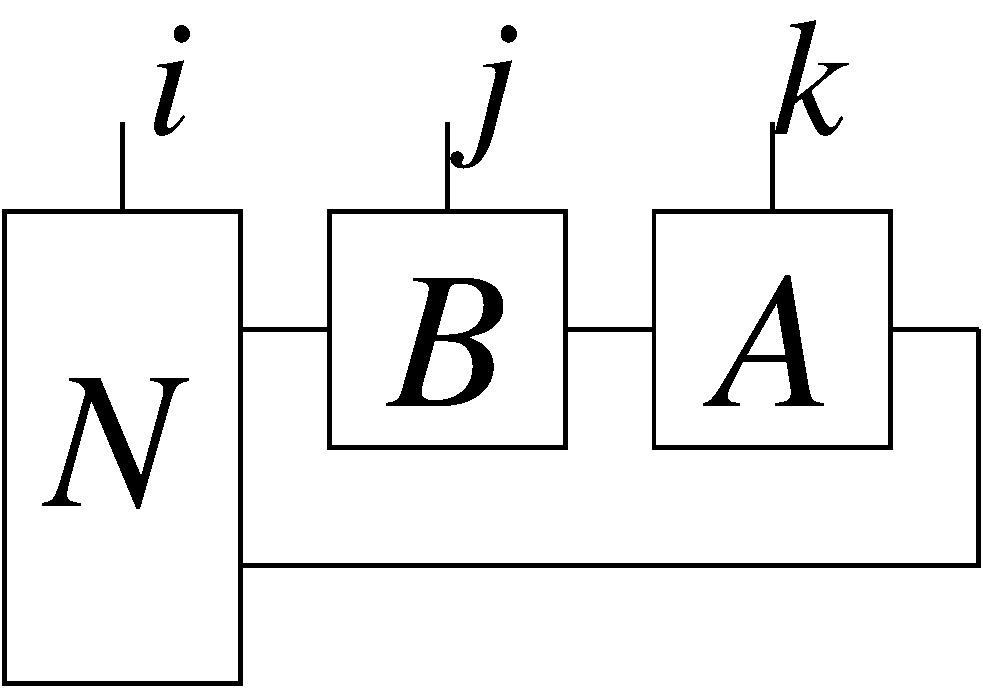
\includegraphics[height=4em]{diagrams/trNBB}}\ .
\]
Apply the inverse of $A$ and $B$ to find a relationship between $M$ and $N$.
Use this relationship to show that $\ket{\psi}$ is contained in the r.h.s., proving inclusion both ways.

\begin{theorem}[Closure property]
\label{thm:closure}
 For injective $A$ and $B$,
\[
    \left\{\raisebox{-1.7em}{\,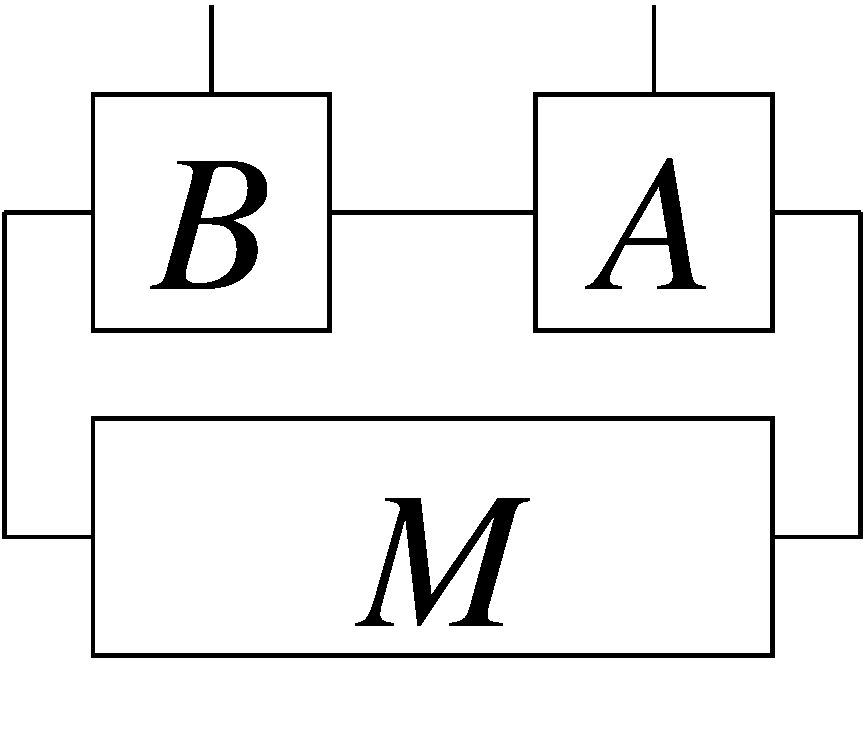
\includegraphics[height=4em]{diagrams/trMBC}}\ \,\middle\vert \ M \right\}
    \cap
    \left\{\raisebox{-1.7em}{\,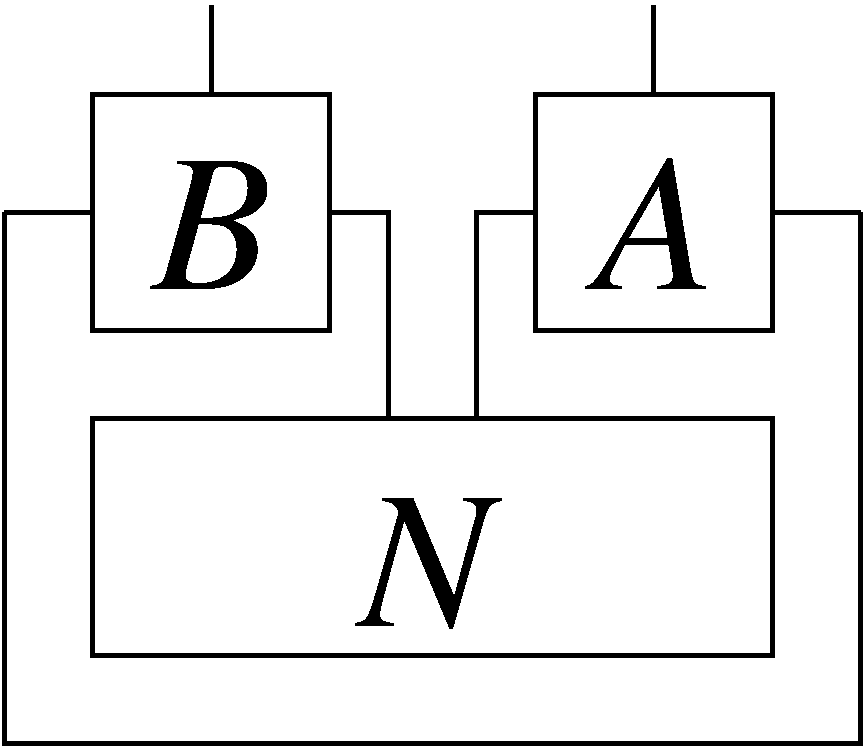
\includegraphics[height=4em]{diagrams/trNBC}}\ \,\middle\vert \ N \right\}=
    \spanset\left\{\raisebox{-.9em}{\,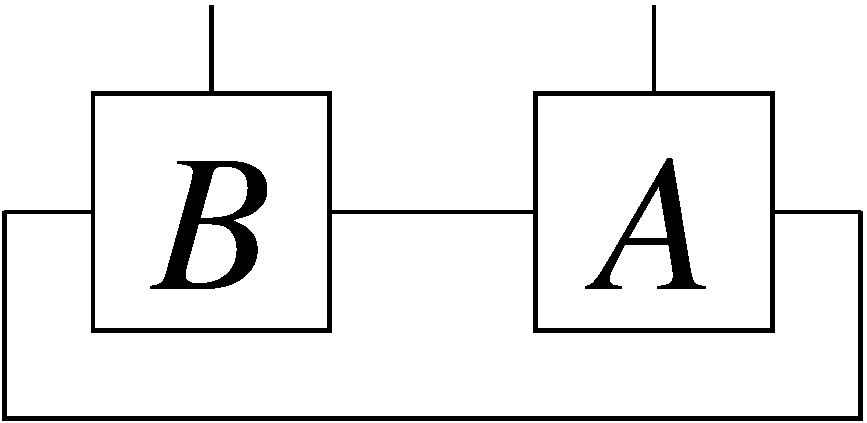
\includegraphics[height=2.5em]{diagrams/trBC}} \right\} \ .
\]
with $M$, $N \in \mathbf{L}(\mathbb{C}^{D \times D})$.
\end{theorem}

As for Theorem~\ref{thm:intersection}, show that the r.h.s. is included in the intersection by choosing $M$ and $N$ appropriately.
To prove inclusion the other way around, take a state belonging to the intersection, apply the inverses, and find that $M \propto \id$, concluding the proof.

We define the operator $h_{i,i+1}$ acting on site $(i,i+1)$
\[
  h_{i,i+1} = \id \otimes (\id - P_{\mathcal{S}_2}) \otimes \id,
\]

where $P_{\mathcal{S}_2}$ is the projector on $\mathcal{S}_2$.
Notice that $\mathcal{S}_2$ is the \emph{ground space} of $h_{i,i+1}$.
Conclude by proving the following theorem.
\begin{theorem}[Parent Hamiltonian]
\label{thm:parent}
Let $A$ be an injective tensor generating an MPS $\ket{\Psi}$. 
There exists a self-adjoint operator $H$, such that $\ket{\Psi}$ is its unique and frustration-free ground state.
\end{theorem}

By induction, use Theorem~\ref{thm:intersection} to prove that the intersection between acting with $h_{i,i+1}$ on every two-body pair $(1,2), (2,3), \dots (L-1,L)$ gives the support of $\mathcal{S}_L$.
Finally, use Theorem~\ref{thm:closure} to prove that acting with the last term $h_{L,1}$ necessarily implies that the only remaining state is 
\[
  \raisebox{-1em}{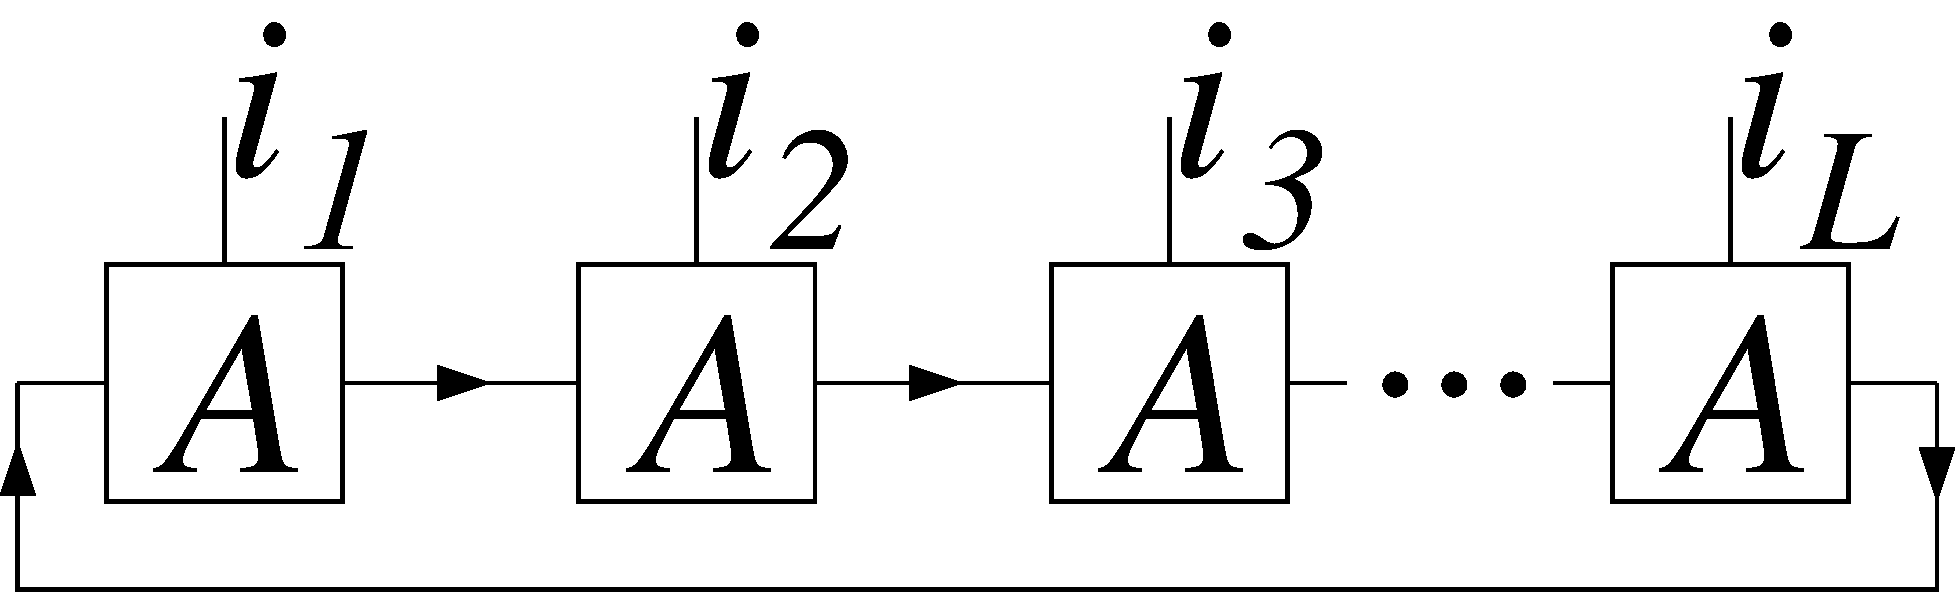
\includegraphics[height=3em]{diagrams/MPS.pdf}} \, = \ket{\Psi}.
\]
\note{Note} This theorem is valid for any injective tensor network.
\end{section}
\end{document}
%%%%%%%%%%% Here Ends Document %%%%%%%%%%
